\section{Experiments}
\label{sec:experiments}

\begin{figure*}[t]
    \centering
    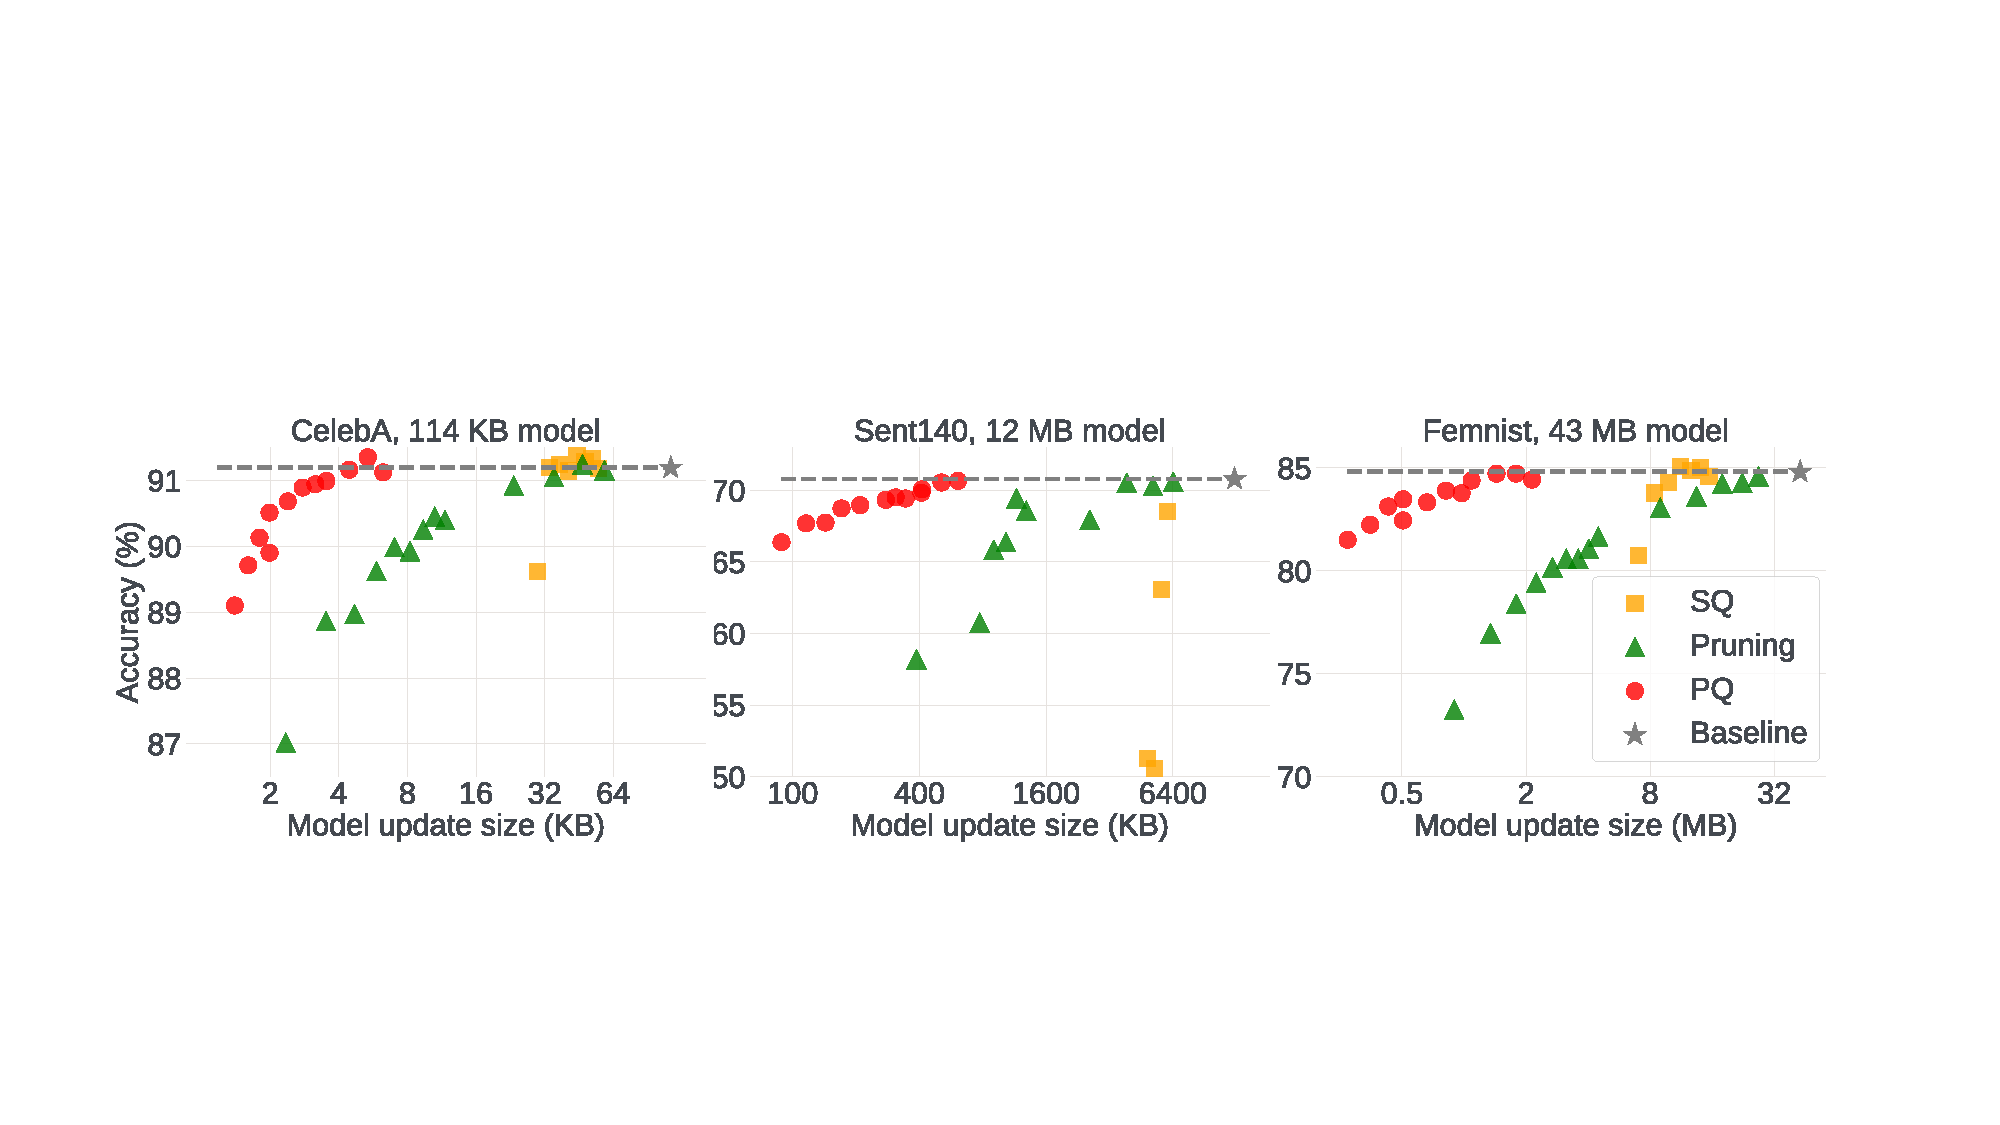
\includegraphics[width=\textwidth]{submissions/GrahamCormode/figs/results_summary.pdf}
    \vspace{-5mm}
    \caption{\label{fig:results_summary}
    We adapt scalar quantization (SQ) and pruning to the \SecAgg protocol to enable efficient and secure uplink communications. We also present results for product quantization (PQ) under the proposed novel \SecInd protocol. \modif{\emph{The $x$ axis is log-scale} and represents the uplink message size}. Baseline refers to \SecAgg FL run without any uplink compression, shown as a horizontal line for easier comparison. Model size is indicated in plot titles. Uncompressed client updates are as large as the models when $p=32$ (see Sec~\ref{subsec:secagg}, shown as stars).
    %We refer to the Appendix~\ref{appendix:table} for the matching tables where we additionally report the standard deviation of each data point.
    }
\end{figure*}

% \pierre{TODO: Table/graph for SQ overflows}
% \pierre{Convergence curves baseline vs compression?}
%In this section, w
We evaluate the performance of the proposed approaches when adapted to \SecAgg protocols.
We study the relationship between uplink compression and model accuracy for the LEAF benchmark tasks.
For scalar and product quantization we also analyze the impact of refresh rate for compression parameters on  model performance.

\subsection{Experimental Setup}
\label{subsec:setup}
We follow the setup of~\cite{nguyen2021federated} and use the {FLSim library}
% \footnote{Available at \href{https://github.com/facebookresearch/FLSim}{https://github.com/facebookresearch/FLSim}}
for our experiments
% \footnote{Code available at \texttt{github.com/facebookresearch/SecureFLCompression}.}
.
All experiments are run on a single V100 GPU 16 GB (except for Sent140 where we use one V100 32 GB) and typically take a few hours to run.
%More experiment details can be found in Appendix \ref{appendix:exp_details}.

\para{Tasks.} We run experiments on three datasets from the LEAF benchmark~\cite{caldas2018leaf}: CelebA~\cite{liu2015faceattributes}, Sent140~\cite{Go_Bhayani_Huang_2009} and FEMNIST~\cite{lecun2010mnist}. For CelebA, we train the same convolutional classifier as ~\cite{nguyen2021federated} with BatchNorm layers replaced by GroupNorm layers and 9,343 clients. For Sent140, we train an LSTM classifier for binary sentiment analysis with $59,400$ clients.
For FEMNIST, we train a GroupNorm version of the ResNet18~\cite{he2015deep} for digit classification with 3,550 clients.
We do not compress biases and norm layers due to their small overhead.

\para{Baselines.}  We focus here on the (synchronous) FedAvg approach although, as explained in Section~\ref{sec:method}, the proposed compression methods can be readily adapted to asynchronous FL aggregation protocols. \modif{As in prior work, we keep the number of clients per round to at most $100$,
%(see Appendix~\ref{appendix:exp_details}),
a small fraction of the total considered population size~\cite{chen2019federated,charles2021largecohort}.}
We report the average and standard deviation of accuracy over three independent runs for all tasks at different uplink byte sizes corresponding to various configurations of the compression operator.
% \sayan{important point : why do we use gradient and client update interchangeably ? they're not the same and for FedAvg it should be client update deltas ?} \karthik {I belieev I have changed gradients to client updates everywhere, except in related works section where we warn we might use graidents to mean updates}

% \subsection{Secure and Efficient Uplink Communications}

\para{Implementation Details.} We refer the reader to \cite{techreport} for full experiment details.
The downlink overhead of sending the per-layer codebooks for product quantization is negligible.
%as shown in Appendix~\ref{appendix:codebook_size}.
The convergence time in terms of rounds is similar for PQ runs and the non-compressed baseline/
%, as illustrated in Appendix~\ref{appendix:convergence}.
Note that outside a simulated environment, the wall-clock time convergence for PQ runs would be \emph{lower} than the baseline since uplink communication would be more efficient, hence faster.

\subsection{Results and Comparison with Prior Work}

Results for efficient and secure uplink communications are displayed in Figure~\ref{fig:results_summary}.
%Note that each method is either design to be adapted to S\SecAgg
We observe that PQ yields a consistently better trade-off curve between model update size and accuracy. For instance, on CelebA, PQ achieves $\times 30$ compression with respect to the non-compressed baseline at iso-accuracy. The iso-accuracy compression rate is $\times 32$ on Sent140 and $\times 40$ on FEMNIST (see~\cite{techreport} for detailed tables).
Scalar quantization accuracy degrades significantly for larger compression rates due to the overflows at aggregation.
%as detailed in Appendix~\ref{appendix:overflow}.
Pruning gives intermediate tradeoffs between scalar quantization and product quantization.

The line of work that develops FL compression techniques is exemplified by FetchSGD~\cite{rothchild2020fetchsgd} as detailed in Section~\ref{sec:related}, where the authors do not address \SecAgg.
Their results are not directly comparable to ours due to incomparable experimental setups (e.g., datasets and architectures).
However, Figure 6~\cite{techreport} mentions upload compression rates at iso-accuracy that are weaker than those obtained here with product quantization.

\subsection{Ablation Studies}
\label{subsec:ablations}

\begin{figure*}[t]
    \label{mask-refresh}
    \centering
    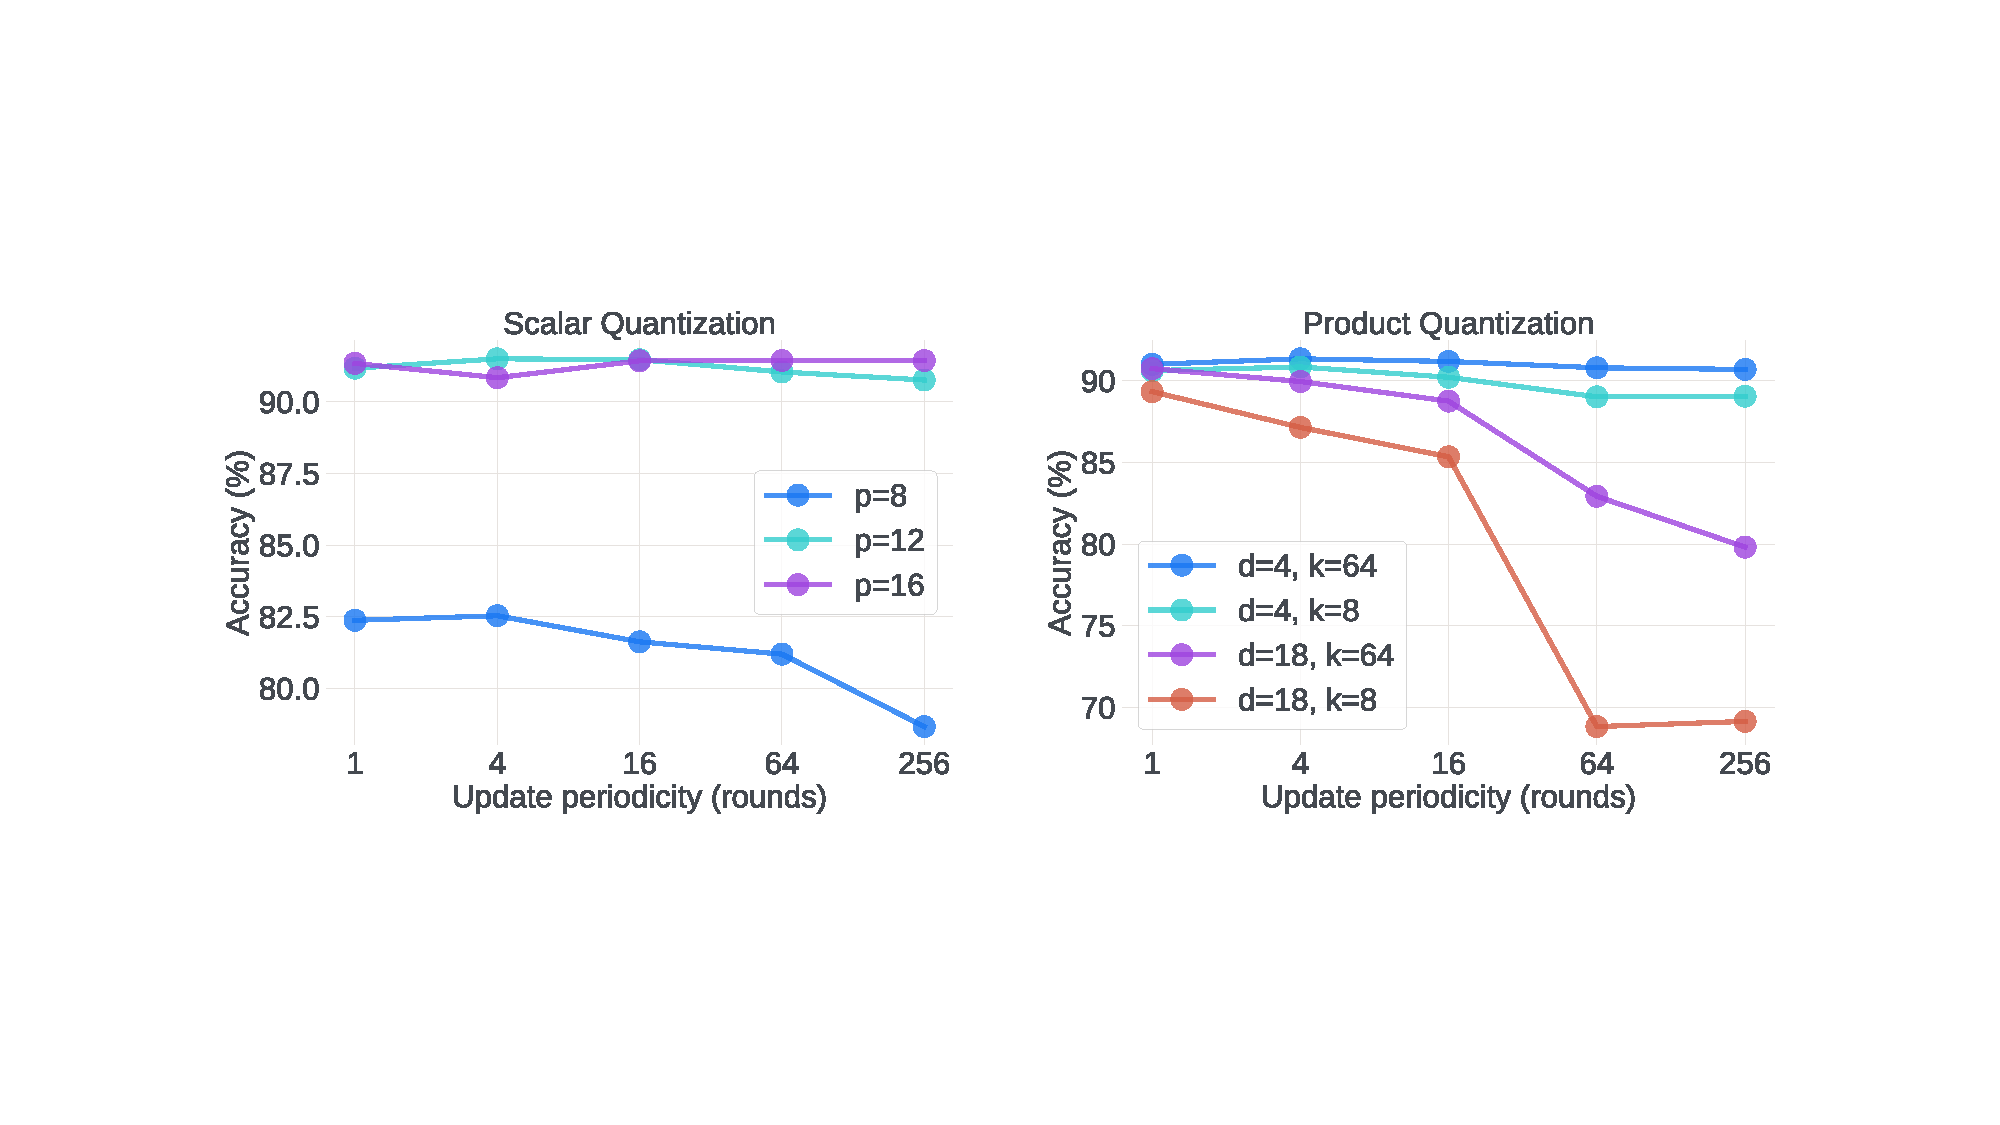
\includegraphics[width=0.9\textwidth]{submissions/GrahamCormode/figs/refresh.pdf}
    \caption{\label{fig:refresh}
    Impact of the refresh rate of the compression operator by the server on the CelebA dataset. \textbf{Left}:  scalar quantization (quantization parameters), fixing the quantization bit-width $b=8$ ($p$ denotes the \SecAgg bit-width). \textbf{Right}: for product quantization (codebooks), where $k$ denotes the number of codewords and $d$ the block size.}
    \vspace{-3mm}
\end{figure*}


We investigate the influence of the frequency of updates of the compression operator $q$ for scalar quantization and pruning, and study the influence of the \SecAgg bit-width $p$ on the number of overflows for scalar quantization.

\para{Update frequency of the compression operators.} In Figure~\ref{fig:refresh}, we show that for scalar quantization, the update periodicity only plays a role with low \SecAgg bit-width values $p$ compared to the quantization bit-width $b$. For product quantization, the update periodicity plays an important role for aggressive compression setups corresponding to large block sizes $d$ or to a smaller number of codewords $k$. For pruning, we measure the impact of masks that are refreshed periodically.
We observed that if we refresh the compression operator more frequently, staleness is reduced, leading to accuracy improvements.
%We present our findings in Appendix~\ref{sparse_refresh}.

\para{Overflows for scalar quantization.}
As discussed in Section~\ref{subsubsec:sq_sa}, we choose the \SecAgg bit-width~$p$ to be greater than quantization bit-width~$b$ in order to avoid aggregation overflows. While it suffices to set $p$ to be $\lceil\log_2 n_c\rceil$ more than $b$, where $n_c$ is the number of clients participating in the round, reducing $p$ is desirable to reduce uplink size.
We studied the impact of  $p$ on the percentage of parameters that suffer overflows, and
observed that there is a benefit to having some non-zero overflow margin size, but no clear correlation between margin size and accuracy.
%present our findings in Appendix~\ref{appendix:overflow}.

% \para{Update frequency of pruning operator $\varrho$.}

% \begin{table*}[t]
%     \small
%     \centering
%     % \vspace{3pt}
%     \begin{tabular}{l@{\hspace{20pt}} c ccc cl@{\hspace{20pt}} ccc}
%     \toprule
%  \bf Compression Method &~~& \multicolumn{3}{c}{\bf CelebA} &~~& \multicolumn{3}{c}{\bf Sent140}\\
%  && \multicolumn{3}{c}{\small ResNet18} &~~& \multicolumn{3}{c}{\small LSTM}\\
% %  && \multicolumn{3}{c}{\small Wikitext-103} &~~& \multicolumn{3}{c}{\small ImageNet-1k}\\
% \cmidrule{3-5}
% \cmidrule{7-9}
% && Gradient size & Compression & Top-1 && Gradient Size & Compression & PPL \\
%     \midrule
%     Baseline & &  $-$ & $\times\ \ 1$ & $-$ & &  $-$ & $\times\ \ 1$ & $-$   \\
%     % \midrule
%     % Binarization & & \\
%     % + \method & & \\
%     \midrule
%     SQ (8 bits) & &  $-$ & $\times\ \ -$ & $-$ & &  $-$ & $\times\ \ -$ & $-$   \\
%     SQ (4 bits) & &  $-$ & $\times\ \ -$ & $-$ & &  $-$ & $\times\ \ -$ & $-$   \\
%     \midrule
%     Pruning ($s=90\%$) & &  $-$ & $\times\ \ -$ & $-$ & &  $-$ & $\times\ \ -$ & $-$   \\
%     Pruning ($s=50\%$) & &  $-$ & $\times\ \ -$ & $-$ & &  $-$ & $\times\ \ -$ & $-$   \\
%     Pruning ($s=10\%$) & &  $-$ & $\times\ \ -$ & $-$ & &  $-$ & $\times\ \ -$ & $-$   \\
%     \midrule
%     PQ ($k=256$, $d=4$) & &  $-$ & $\times\ \ -$ & $-$ & &  $-$ & $\times\ \ -$ & $-$   \\
%     PQ ($k=256$, $d=8$) & &  $-$ & $\times\ \ -$ & $-$ & & $-$ &  $\times\ \ -$ &  $-$  \\
%     \bottomrule
%     \end{tabular}
%  \caption{\small \textbf{Comparison of different quantization schemes with Secure Aggregation}. Blabla.}
%     \label{tab:quantization_comparison}
% \end{table*}


% \subsection{Combination of Compression Techniques}

% \pierre{Song Han Deep Compression for combination}

% \subsubsection{Sparsity \& Scalar Quantization}
% Say/demonstrate that its better to perform pruning first and then SQ than the opposite.

% \subsubsection{Sparsity \& Product Quantization}
% Block sparsity and PQ.

% \subsection{FL Finetuning}

% Maybe also talk about the realistic scenario of FL finetuning (in practice, start from pretrained model on public data to bootstrap learning, in which case gradients may be smaller/sparser hence easier to compress?).
% Partial finetuning.

% \subsection{Heterogeneous Hardware}

% Experiment describing various bit-widths/sparsity level/codebook size per client depending on available bandwidth.

% \pierre{delta with respect to baseline}
% \pierre{discussion about privacy of shared parameters}
% \pierre{DP noise in the enclave until the very end. Privacy vs security = secure FL focus}
% \pierre{Secure Coding} 